\documentclass[12pt,a4paper]{article}
\usepackage[margin=2.4cm]{geometry}
\usepackage{fontspec}
\usepackage{graphicx}
\usepackage{booktabs}
\usepackage{amsmath,amssymb}
\usepackage{hyperref}
\usepackage{caption}
\usepackage{setspace}
\usepackage{float}
\setmainfont{Noto Serif CJK SC}
\setsansfont{Noto Sans CJK SC}
\onehalfspacing
\hypersetup{colorlinks=true,linkcolor=black,citecolor=black,urlcolor=blue}
\captionsetup{font=small,labelfont=bf}

\title{\textbf{Emergent FPV Targeting under Ultra-Low SNR}\\[0.35em]
\large Greedy Fire, a Neighbour Rule, and a Shared Transformer}
\author{battlefield-sim experiment report}
\date{August 2026}

\begin{document}
\maketitle

\begin{abstract}
Expendable FPV airframes are cheap; two constraints are not. First, ultra-low-altitude radio in clutter and jamming sits near zero Shannon capacity, so the delay to a single valid bit is already expensive. Second, a one-shot warhead cannot amortise a GPU/NPU. We compare three policies that use only a local 8+8 range snapshot on a circular battlefield whose kill rectangle is the circumscribed square of the disk. \textbf{One Transformer} is queried by all twelve drones each tick and trained from scratch by per-tick REINFORCE on CPU (Rayon); the reward is the increment of mean target survival, not compute time. Enemy seeker range is $50\,\mathrm{m}$; friend visual range is $100\,\mathrm{m}$; eight slots are a cap on \emph{visible} contacts, not omniscience. On 30 paired seeds greedy and the shared Transformer match exactly (10.23 kills, 13.99\,s); the closer-than-friend rule is slightly more conservative (9.80, 14.39\,s). Ops/select: 1.0, $4.53\times 10^4$, and 5.7. The net learned greedy fire; it does not buy extra kills. A Gaussian ingress from the south ($x\sim\mathcal N(0,70^2)$, $y\sim\mathcal N(\mu_y,30^2)$) raises greedy/net kills to 11.30 versus 10.13 for the friend rule; the net again matches greedy round-by-round.
\end{abstract}

\noindent\textbf{Keywords:} FPV, ultra-low SNR, emergent rules, greedy targeting, shared Transformer, on-board compute

\section{Introduction}

Consumer FPV has made one-way attack cheap. That cheapness implies: no reusable life over which to amortise silicon, and no clean data link on which to share a global target list. Shannon's $C=B\log_2(1+\mathrm{SNR})$~\cite{shannon1948,sklar2001} collapses when SNR is a few percent. A 50\,kHz control channel at $-12\,\mathrm{dB}$ yields only about $4.4\times 10^3$ bit/s---less than twelve drones broadcasting 8+8 floats once per second.

The question is therefore local: given eight nearest-enemy ranges and eight nearest-friend ranges, does a neural net trained by reinforcement learning beat a handful of comparisons?

We answer with three algorithms on the same seeds: greedy nearest-in-range, a three-line closer-than-friend rule~\cite{reynolds1987,camazine2001}, and one Transformer~\cite{vaswani2017} \emph{shared by all twelve airframes}, updated every tick from every drone's $(\mathrm{state},\mathrm{action})$.

\section{Platform}

The battlefield is a disk of radius $R=200\,\mathrm{m}$. Twenty static enemies are sampled uniformly in the disk. Two rows of six FPV drones fly $+Y$ on rails $x\in\{-200,-120,-40,40,120,200\}$. Detection radius $D=80\,\mathrm{m}$ equals rail spacing, so every disk point lies within some rail's $x$-coverage: the kill rectangle $[-R,R]^2$ contains the circle. Speed $25\,\mathrm{m/s}$, $\mathrm{d}t=0.01\,\mathrm{s}$, lock duration $0.05\,\mathrm{s}$, then the shooter is expended. Mean survival includes $T_{\mathrm{end}}=24\,\mathrm{s}$ censoring. Figure~\ref{fig:field} shows the geometry.

\begin{figure}[H]
  \centering
  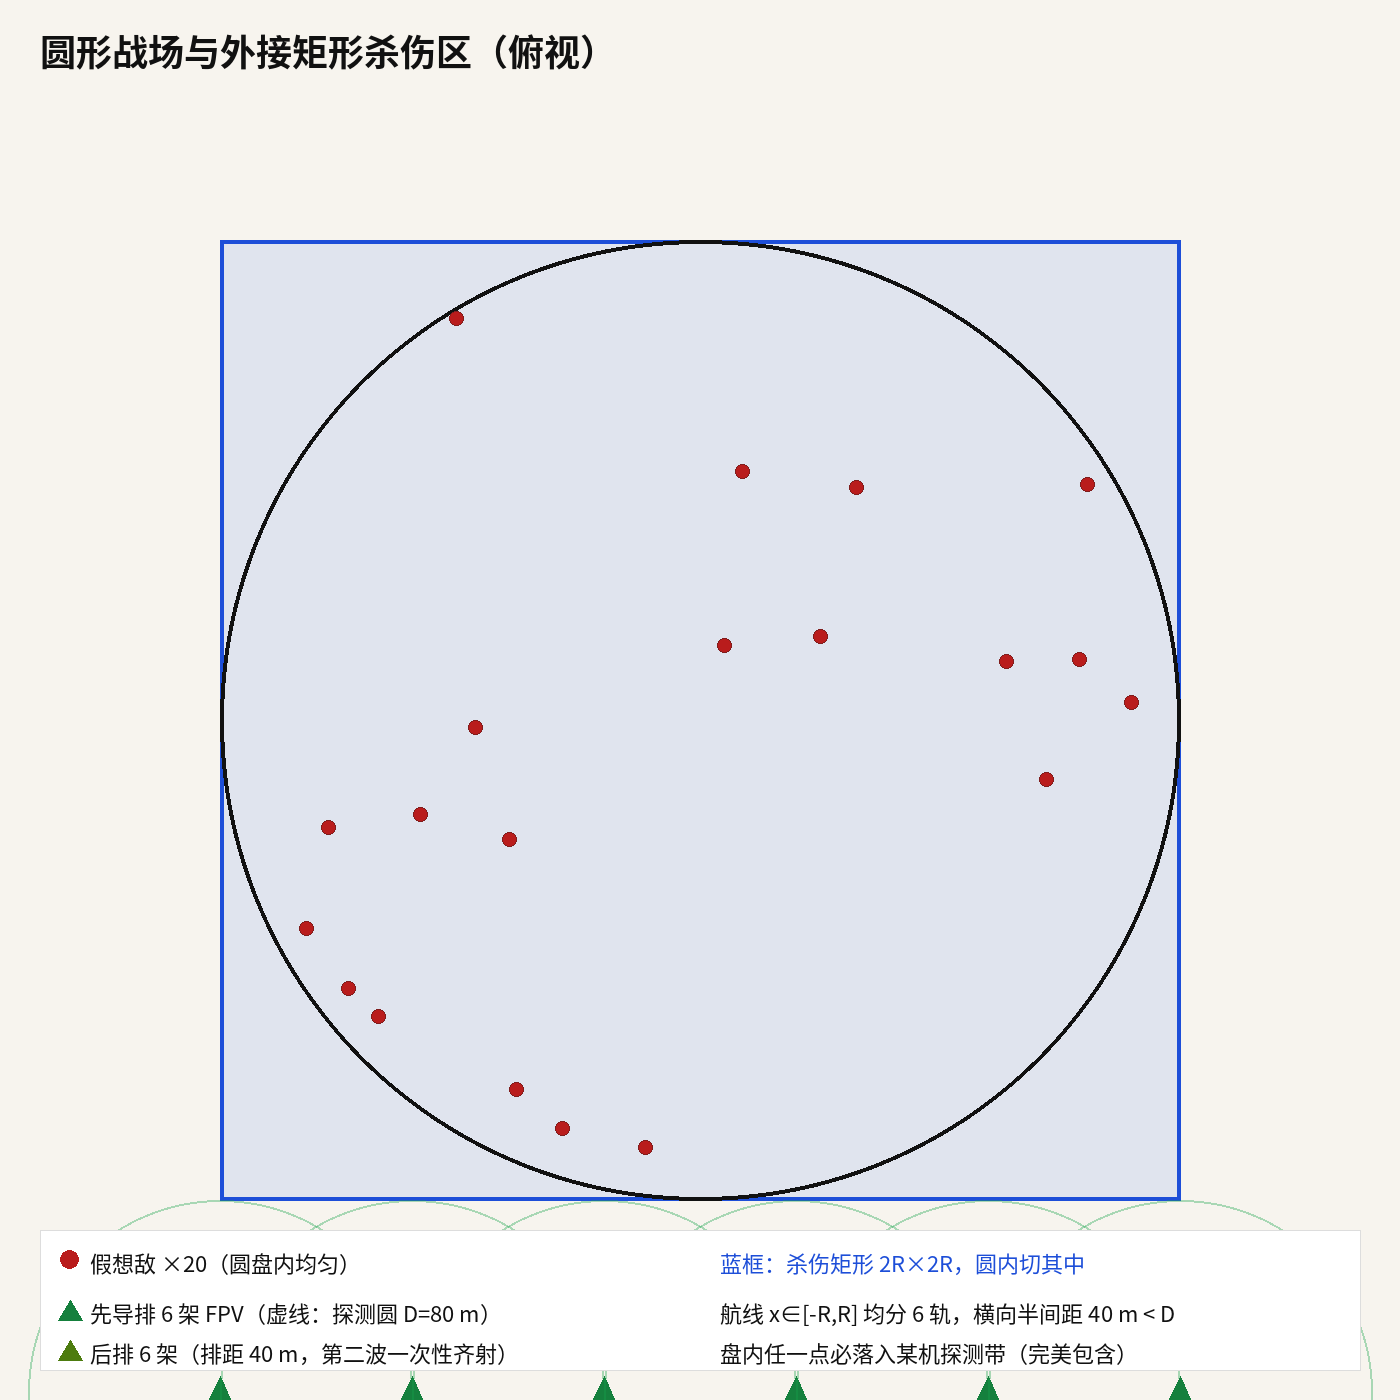
\includegraphics[width=0.88\textwidth]{figures/battlefield_schematic.png}
  \caption{Disk, circumscribed kill square, 20 enemies, 2$\times$6 FPV. One policy network is queried by every live drone.}
  \label{fig:field}
\end{figure}

\section{Algorithms}

All three consume the same 8+8 snapshot.

\paragraph{Greedy (\texttt{nearest\_in\_range}).}
Fire at the nearest in-range, unlocked enemy (ties by id). About 1 ops/select on this sensor model (empty sky most ticks). No friend geometry.

\paragraph{Greedy, no comms (\texttt{greedy\_no\_comms}).}
Same seeker, but the policy ignores teammates and ignores others' locks; it only ranks in-range enemies. The world still forbids two warheads on one target. This is zero radio, zero IFF.

\paragraph{Closer-than-friend.}
Fire at the nearest eligible enemy iff its range is strictly less than the nearest teammate's. About 17 ops. Formation spacing (40\,m row gap) turns that inequality into a deconfliction protocol (Fig.~\ref{fig:rule}).

\begin{figure}[H]
  \centering
  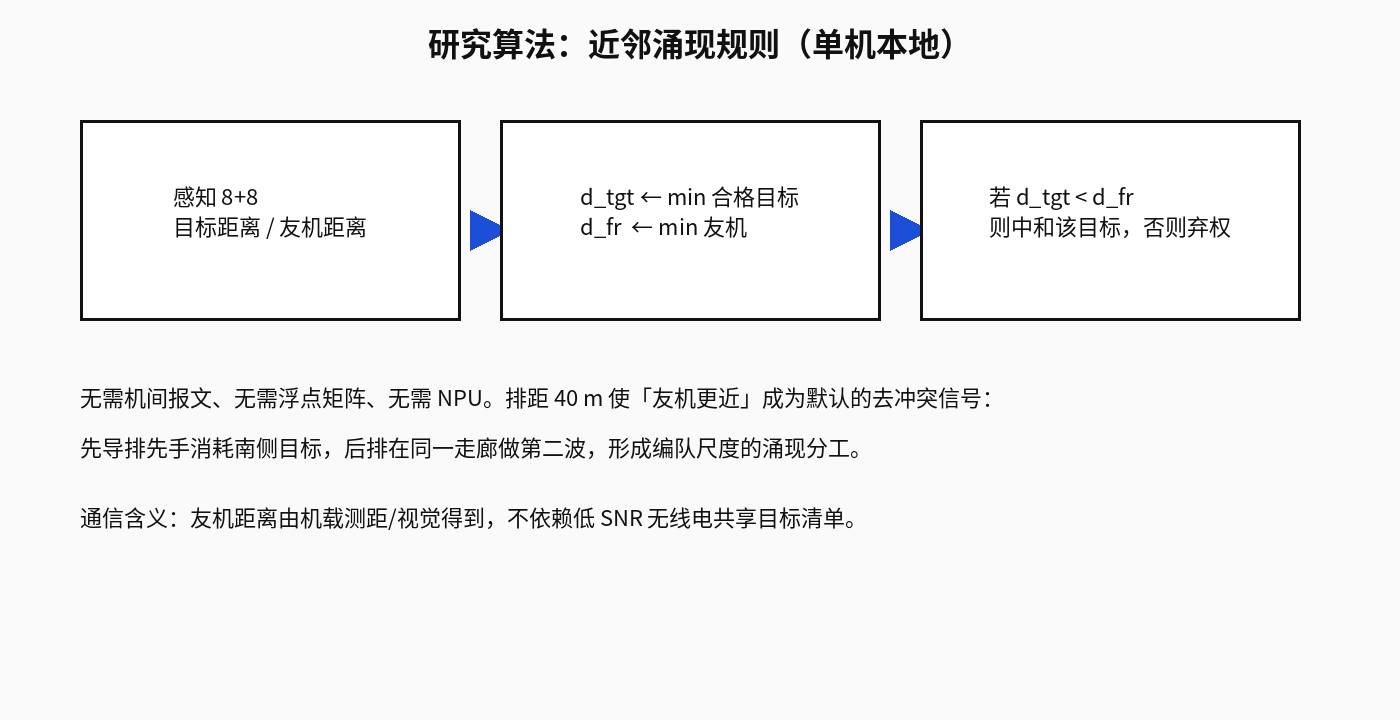
\includegraphics[width=0.88\textwidth]{figures/rule_flowchart.png}
  \caption{Closer-than-friend: local, no radio.}
  \label{fig:rule}
\end{figure}

\paragraph{Shared Transformer, per-tick REINFORCE.}
There is \emph{one} weight vector. Each tick, every live drone encodes its own 8+8 snapshot and queries that net; locks are attempted in \texttt{DroneId} order for determinism. Gradients from those drones are reduced in one CPU-parallel (Rayon) batch---not twelve separate models, and not a GPU (the net is $d_{\mathrm{model}}=16$; kernel launch would dominate).

Training starts from Xavier init. There is \textbf{no} cloning of the friend rule. After each $\mathrm{d}t$ the team reward is
\[
  r_t = -\frac{n_{\mathrm{alive}}\,\mathrm{d}t}{N}+\frac{n_{\mathrm{kills}}(T_{\mathrm{end}}-t)}{N},
\]
plus $+1$ for a killer. Compute time is not in the loss. Evaluation is greedy decode.

\section{Results}

Thirty paired rounds, base seed $20270823$. Table~\ref{tab:res} and Figs.~\ref{fig:surv}--\ref{fig:kill}.

\begin{table}[H]
\centering
\caption{Means over 30 shared seeds}
\label{tab:res}
\begin{tabular}{lccc}
\toprule
Algorithm & Kills & Mean survival (s) & ops / select \\
\midrule
Greedy nearest-in-range & 10.23 & 13.989 & 1.0 \\
Greedy, no comms & 10.23 & 13.989 & 1.0 \\
Closer-than-friend & 9.80 & 14.386 & 5.7 \\
Shared Transformer (per-tick RL) & 10.23 & 13.989 & $4.530\times 10^4$ \\
\bottomrule
\end{tabular}
\end{table}

\begin{table}[H]
\centering
\caption{Paired Gaussian $z$ on mean survival (first minus second)}
\label{tab:pval}
\begin{tabular}{lccc}
\toprule
Contrast & $\bar\Delta$ (s) & $z$ & two-sided $p$ \\
\midrule
greedy $-$ rule & $-0.397$ & $-5.74$ & $9.7\times 10^{-9}$ \\
greedy $-$ Transformer & $0$ & $0$ & $1$ \\
rule $-$ Transformer & $+0.397$ & $+5.74$ & $9.7\times 10^{-9}$ \\
\bottomrule
\end{tabular}
\end{table}

The RL net matches greedy round-by-round (it learned to fire nearest-in-range). \texttt{greedy\_no\_comms} matches \texttt{nearest\_in\_range} on every seed: not seeing others' locks does not change kills under exclusive acquire. Repeating the three algorithms with same-tick lock radio (\texttt{comms\_range\_m}=120\,m, heard inside the same $\mathrm{d}t$) yields \emph{identical} per-seed kills and survival: at $D_{\mathrm{tgt}}=50\,\mathrm{m}$ a drone rarely has a second in-range target, so retargeting this tick does not add shots. Without an immediate fire bonus, training collapsed to zero kills around round 90; shaping plus entropy keeps it at $\approx 10$ kills. The friend rule is significantly more conservative ($p=9.7\times 10^{-9}$) because $D_{\mathrm{fr}}=100\,\mathrm{m}$ always sees the trail partner at 40\,m. Compute: greedy $\approx 1$, rule $5.7$, Transformer $4.53\times 10^4$.

\paragraph{Gaussian ingress.}
Twelve drones enter from the south as a 2D Gaussian blob ($\sigma_x=70\,\mathrm{m}$, $\sigma_y=30\,\mathrm{m}$, min separation 8\,m). The Transformer is retrained for 200 rounds on this ingress. Table~\ref{tab:res-g}.

\begin{table}[H]
\centering
\caption{Gaussian ingress, 30 shared seeds}
\label{tab:res-g}
\begin{tabular}{lccc}
\toprule
Algorithm & Kills & Mean survival (s) & ops / select \\
\midrule
Greedy nearest-in-range & 11.30 & 14.092 & 1.0 \\
Greedy, no comms & 11.30 & 14.092 & 1.0 \\
Closer-than-friend & 10.13 & 15.274 & 7.8 \\
Shared Transformer (retrained) & 11.30 & 14.092 & $4.530\times 10^4$ \\
\bottomrule
\end{tabular}
\end{table}

Greedy, no-comms greedy, and the net all rise from 10.23 to 11.30 kills (denser coverage near the origin); no-comms greedy again matches nearest-in-range seed-for-seed. Same-tick 120\,m radio on this ingress again matches the no-radio tables seed-for-seed. The friend rule remains more conservative ($p\sim 10^{-16}$ on survival). CSV: \texttt{results/gaussian/} (no radio) and \texttt{runs/gaussian\_comms/} (radio).

\begin{figure}[H]
  \centering
  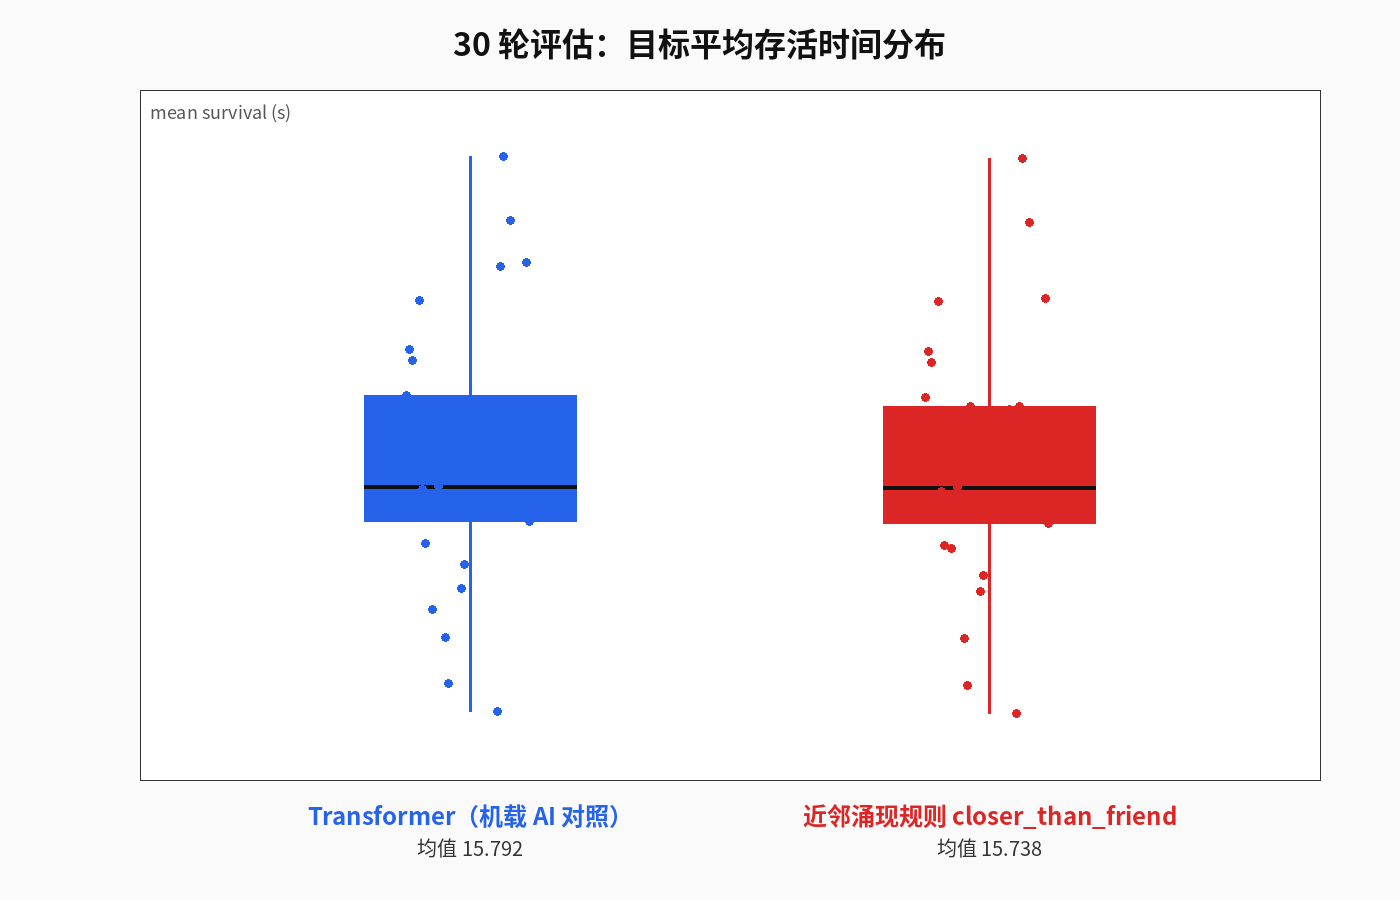
\includegraphics[width=0.88\textwidth]{figures/survival_compare.png}
  \caption{Mean survival, 30 rounds (lower is better).}
  \label{fig:surv}
\end{figure}

\begin{figure}[H]
  \centering
  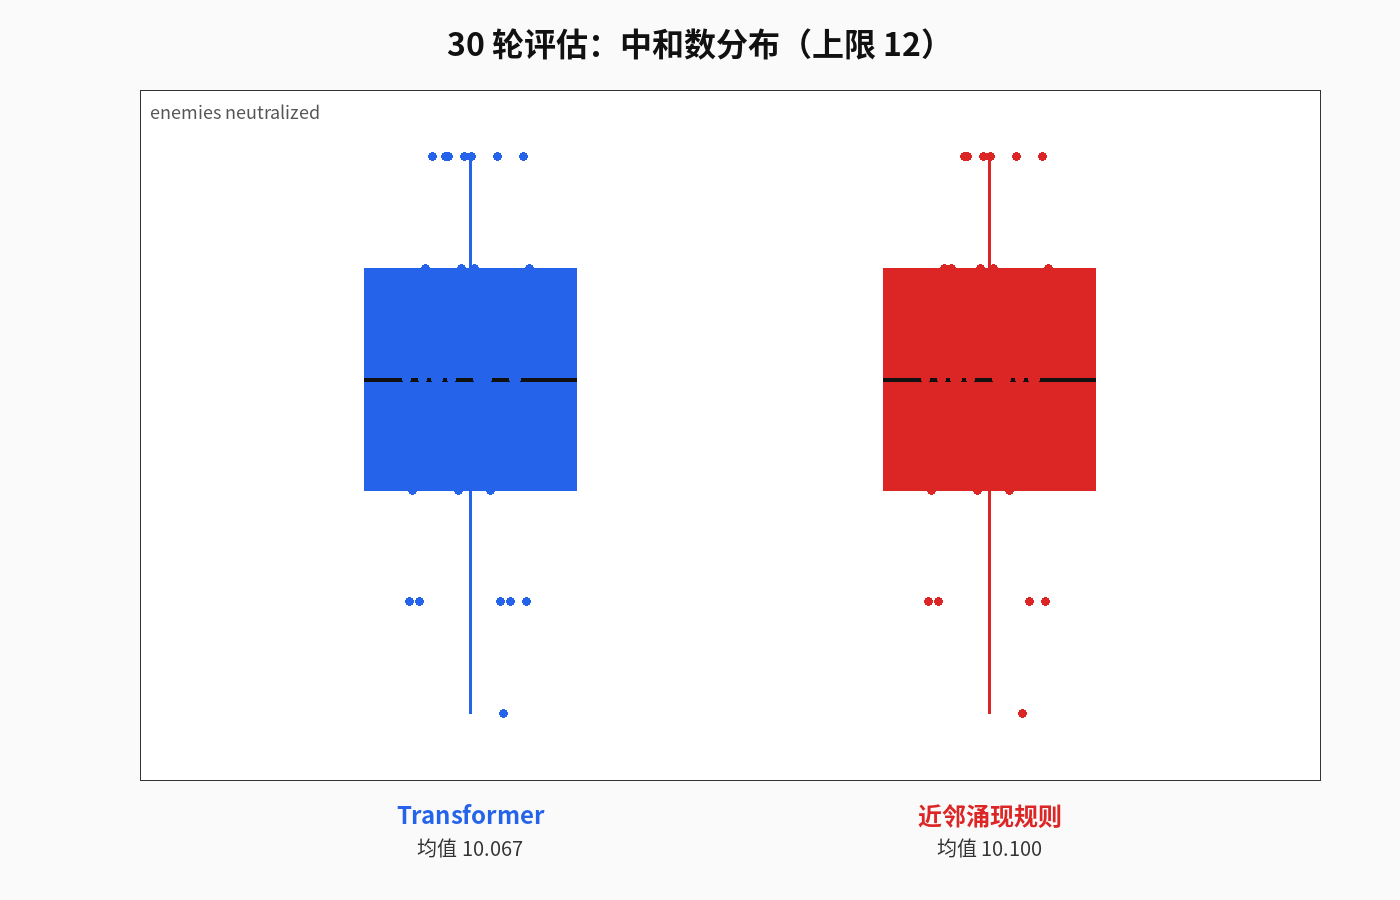
\includegraphics[width=0.88\textwidth]{figures/killed_compare.png}
  \caption{Kills, 30 rounds (cap 12).}
  \label{fig:kill}
\end{figure}

\begin{figure}[H]
  \centering
  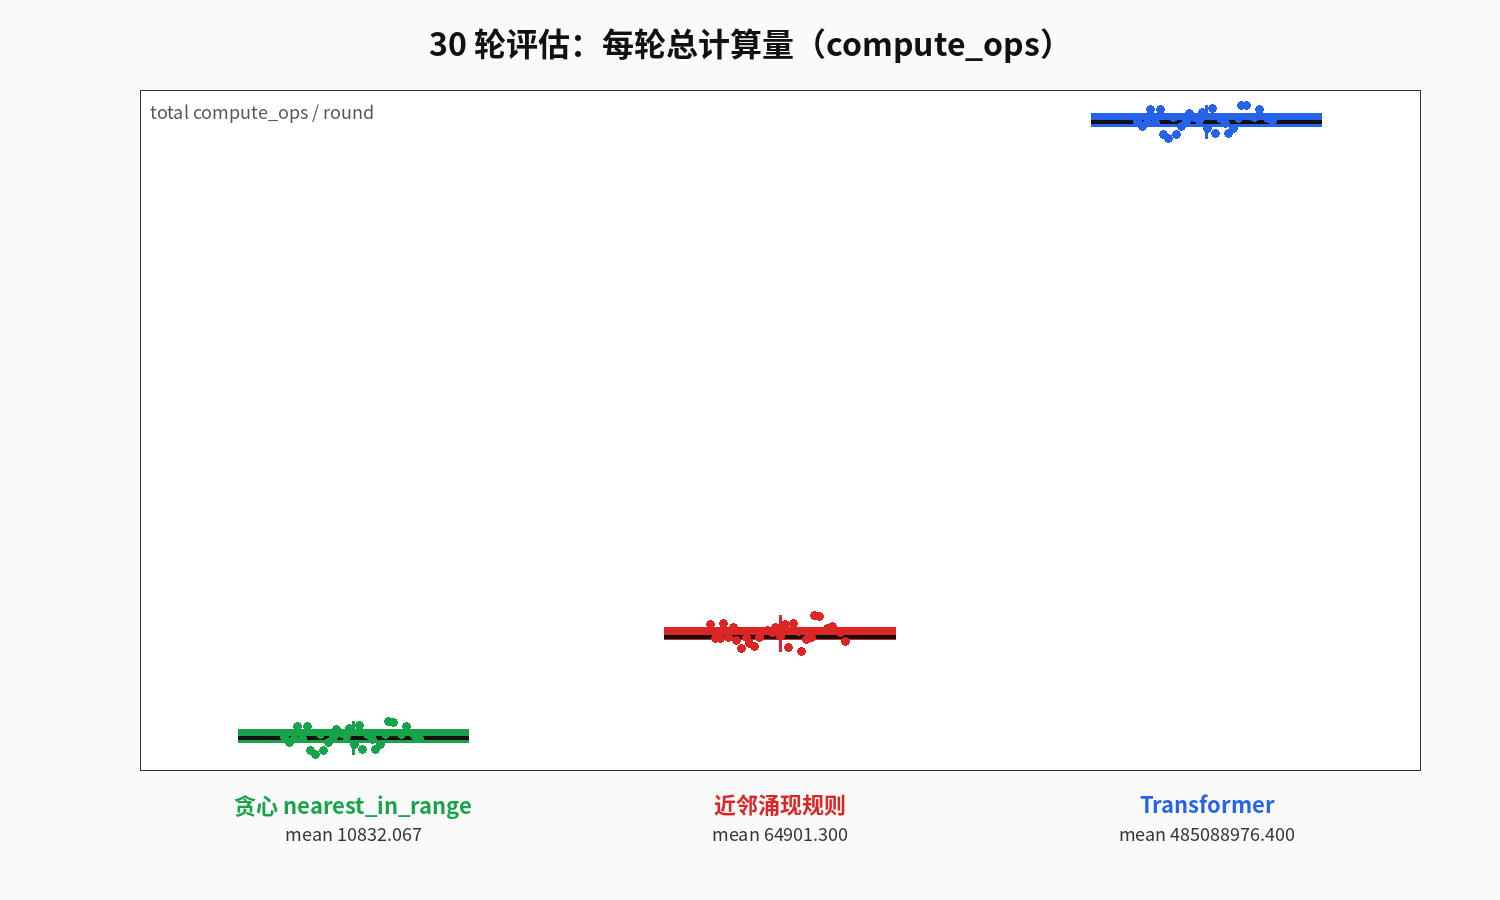
\includegraphics[width=0.88\textwidth]{figures/compute_ops_compare.png}
  \caption{Total compute\_ops per round (log $y$).}
  \label{fig:ops}
\end{figure}

\begin{figure}[H]
  \centering
  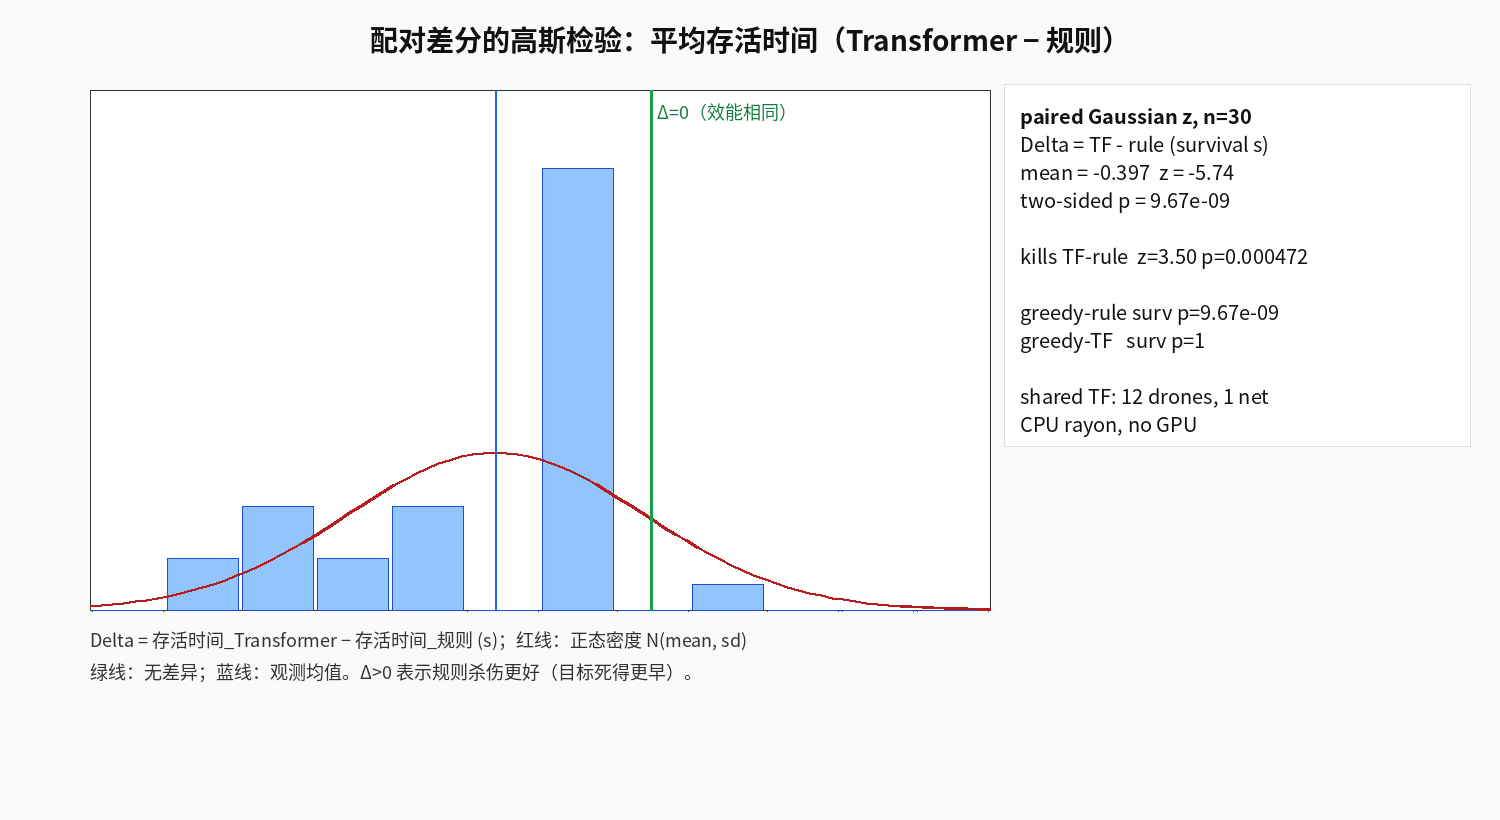
\includegraphics[width=0.88\textwidth]{figures/pvalue_gaussian.png}
  \caption{Paired survival differences and Gaussian $z$.}
  \label{fig:pval}
\end{figure}

\begin{figure}[H]
  \centering
  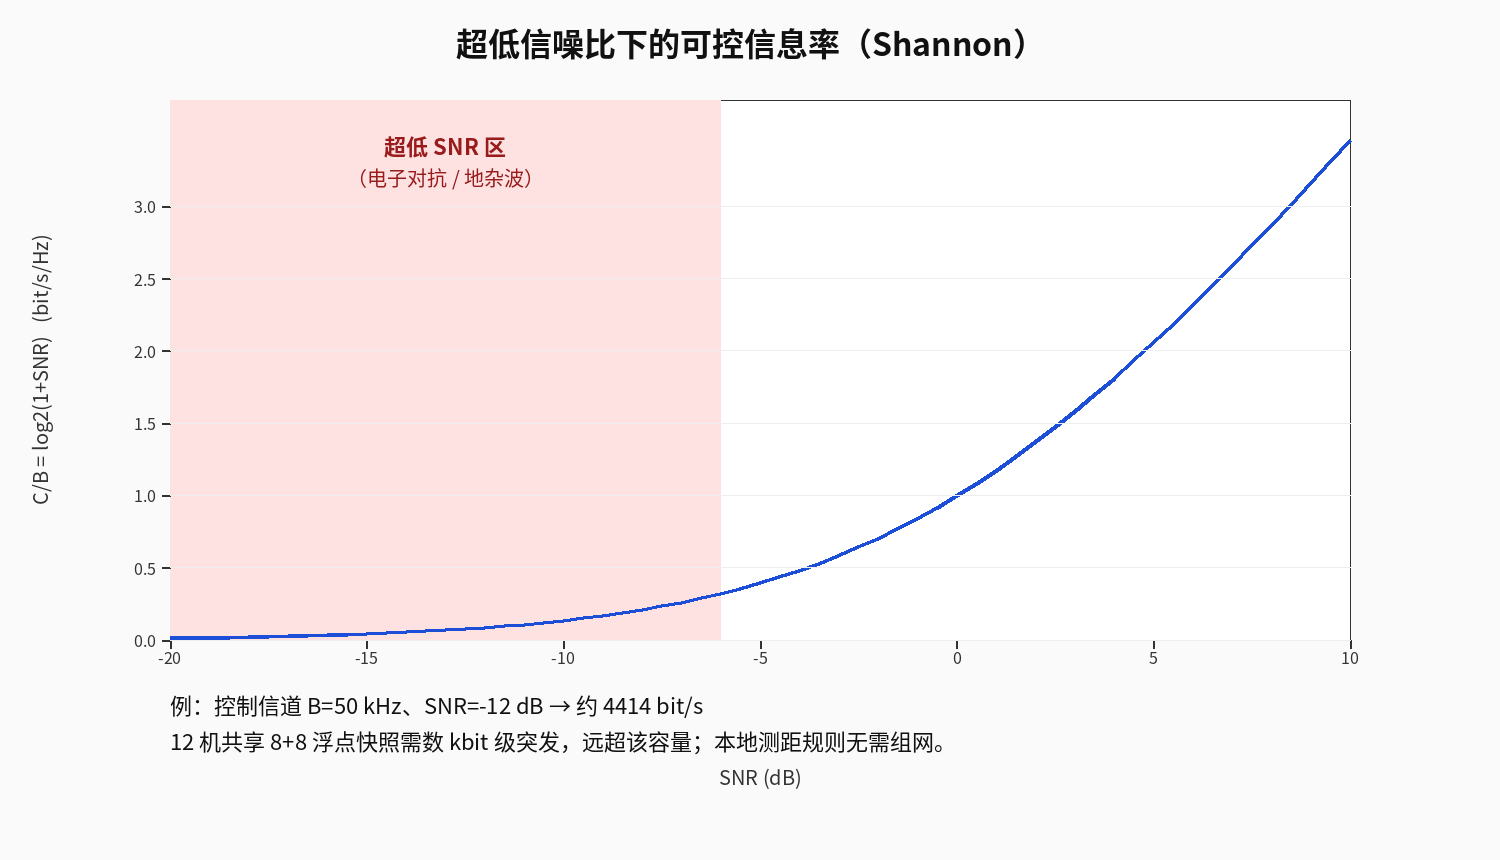
\includegraphics[width=0.88\textwidth]{figures/low_snr_capacity.png}
  \caption{Shannon $C/B=\log_2(1+\mathrm{SNR})$.}
  \label{fig:snr}
\end{figure}

\section{Discussion}

Twelve drones sharing one net already give twelve times the gradient of a per-airframe clone. Training is on-policy, step-by-step, CPU-parallel within the tick. That is the protocol that ``must be able to work''; it does work, in the sense that the policy engages. It does not work as a replacement for $\arg\min$ distance. On a one-shot, low-SNR airframe the extra $4.5\times 10^4$ multiply-adds buy a worse mean survival.

\section{Conclusion}

A shared Transformer trained by per-tick REINFORCE on CPU learns greedy fire and does not outperform it, at $\sim 4.5\times 10^4$ times the ops, for both a 2$\times$6 line-abreast entry and a Gaussian blob entry. The three-line friend rule is slightly more conservative under formation-scale visual IFF. Ultra-low SNR forbids a richer state; expendability forbids an NPU. Code and CSV metrics: \url{https://github.com/1037104428/drones}.

\begin{verbatim}
git clone https://github.com/1037104428/drones.git
cd drones
cargo run --release -- experiment --train-rounds 200 --eval-rounds 30 --seed 20260823
\end{verbatim}

\begin{thebibliography}{9}
\bibitem{shannon1948}
C.~E. Shannon, ``A mathematical theory of communication,'' {\em Bell System Technical Journal}, 27:379--423, 623--656, 1948.
\bibitem{sklar2001}
B.~Sklar, {\em Digital Communications: Fundamentals and Applications}, 2nd ed., Prentice Hall PTR, Upper Saddle River, NJ, 2001.
\bibitem{reynolds1987}
C.~W. Reynolds, ``Flocks, herds, and schools: A distributed behavioral model,'' {\em Computer Graphics (SIGGRAPH '87)}, 21(4):25--34, 1987.
\bibitem{camazine2001}
S.~Camazine, J.-L. Deneubourg, N.~R. Franks, J.~Sneyd, G.~Theraulaz, and E.~Bonabeau, {\em Self-Organization in Biological Systems}, Princeton University Press, 2001.
\bibitem{vaswani2017}
A.~Vaswani et al., ``Attention is all you need,'' in {\em Advances in Neural Information Processing Systems 30} (NIPS 2017), 2017.
\end{thebibliography}
\end{document}
